\documentclass[12pt,letterpaper]{article}
\usepackage{graphicx,textcomp}
\usepackage{natbib}
\usepackage{setspace}
\usepackage{fullpage}
\usepackage{color}
\usepackage[reqno]{amsmath}
\usepackage{amsthm}
\usepackage{fancyvrb}
\usepackage{amssymb,enumerate}
\usepackage[all]{xy}
\usepackage{endnotes}
\usepackage{lscape}
\newtheorem{com}{Comment}
\usepackage{float}
\usepackage{hyperref}
\newtheorem{lem} {Lemma}
\newtheorem{prop}{Proposition}
\newtheorem{thm}{Theorem}
\newtheorem{defn}{Definition}
\newtheorem{cor}{Corollary}
\newtheorem{obs}{Observation}
\usepackage[compact]{titlesec}
\usepackage{dcolumn}
\usepackage{tikz}
\usetikzlibrary{arrows}
\usepackage{multirow}
\usepackage{xcolor}
\newcolumntype{.}{D{.}{.}{-1}}
\newcolumntype{d}[1]{D{.}{.}{#1}}
\definecolor{light-gray}{gray}{0.65}
\usepackage{url}
\usepackage{listings}
\usepackage{color}
\usepackage{layouts}

\definecolor{codegreen}{rgb}{0,0.6,0}
\definecolor{codegray}{rgb}{0.5,0.5,0.5}
\definecolor{codepurple}{rgb}{0.58,0,0.82}
\definecolor{backcolour}{rgb}{0.95,0.95,0.92}

\lstdefinestyle{mystyle}{
	backgroundcolor=\color{backcolour},   
	commentstyle=\color{codegreen},
	keywordstyle=\color{magenta},
	numberstyle=\tiny\color{codegray},
	stringstyle=\color{codepurple},
	basicstyle=\footnotesize,
	breakatwhitespace=false,         
	breaklines=true,                 
	captionpos=b,                    
	keepspaces=true,                 
	numbers=left,                    
	numbersep=5pt,                  
	showspaces=false,                
	showstringspaces=false,
	showtabs=false,                  
	tabsize=2
}
\lstset{style=mystyle}
\newcommand{\Sref}[1]{Section~\ref{#1}}
\newtheorem{hyp}{Hypothesis}

\title{Problem Set 2}
\date{Due: October 23, 2025}
\author{Applied Stats/Quant Methods 1}

\begin{document}
	\maketitle
	\section*{Instructions}
	\begin{itemize}
		\item Please show your work! You may lose points by simply writing in the answer. If the problem requires you to execute commands in \texttt{R}, please include the code you used to get your answers. Please also include the \texttt{.R} file that contains your code. If you are not sure if work needs to be shown for a particular problem, please ask.
		\item Your homework should be submitted electronically on GitHub.
		\item This problem set is due before 23:59 on Thursday October 23, 2025. No late assignments will be accepted.
		
	\end{itemize}
	
	
	\vspace{.5cm}
	\section*{Question 1: Political Science}
	\vspace{.25cm}
	The following table was created using the data from a study run in a major Latin American city.\footnote{Fried, Lagunes, and Venkataramani (2010). ``Corruption and Inequality at the Crossroad: A Multimethod Study of Bribery and Discrimination in Latin America. \textit{Latin American Research Review}. 45 (1): 76-97.} As part of the experimental treatment in the study, one employee of the research team was chosen to make illegal left turns across traffic to draw the attention of the police officers on shift. Two employee drivers were upper class, two were lower class drivers, and the identity of the driver was randomly assigned per encounter. The researchers were interested in whether officers were more or less likely to solicit a bribe from drivers depending on their class (officers use phrases like, ``We can solve this the easy way'' to draw a bribe). The table below shows the resulting data.
	
	\newpage
	\begin{table}[h!]
		\centering
		\begin{tabular}{l | c c c }
			& Not Stopped & Bribe requested & Stopped/given warning \\
			\\[-1.8ex] 
			\hline \\[-1.8ex]
			Upper class & 14 & 6 & 7 \\
			Lower class & 7 & 7 & 1 \\
			\hline
		\end{tabular}
	\end{table}
	
	\begin{enumerate}
		
		\item [(a)]
		Calculate the $\chi^2$ test statistic by hand/manually (even better if you can do "by hand" in \texttt{R}).\\
		
		\noindent \textbf{Step 1: Put the data in R and calculate the totals}
		
		\noindent First I put the tabular data into a matrix. The table without totals or labels was named observed\_table. Then I added the row and column totals and labeled the matrix the same way the original table was labeled. I named the table with the totals and labels class\_table
		
		\lstinputlisting[language=R, firstline=7, lastline=28]{PS02_answersKC.R}  
	
	\begin{center}
		\begin{verbatim}
             Not Stopped Bribe Requested Stoped/Given Warning Row Total
Upper Class           14               6                    7        27
Lower Class            7               7                    1        15
Column Total          21              13                    8        42
		\end{verbatim}
	\end{center}
		
		\newpage
		
		\noindent \textbf{Step 2: Calculate the expected values}
		
		\noindent Find the expected values by calculating row total/grand total * column total
		
		\lstinputlisting[language=R, firstline=31, lastline=46]{PS02_answersKC.R}  
		
		\begin{verbatim}
            Not Stopped Bribe Requested Stopped/Given Warning
Upper Class        13.5        8.357143              5.142857
Lower Class         7.5        4.642857              2.857143
		\end{verbatim}

	\noindent \textbf{Step 3: Assumptions}
\begin{itemize}
	\item The data is categorical
	\item The observations are independent
	\item The groups are mutually exclusive
	\item All of the expected counts are at least 5 (that isn't met in this example)
\end{itemize}

\noindent \textbf{Step 4: State hypotheses}

\begin{itemize}
	\item Null Hypothesis: The variables are statistically independent
	\item Alternative Hypothesis: The variables are statistically dependent
\end{itemize}

		\noindent \textbf{Step 5: Calculate the Chi Squared Statistic} 
		
		\noindent Calculate the Chi-Squared Statistic by taking the (observed values minus the expected values) squared, then dividing that by the expected value. Do that for every value in the table then sum all of them together
		
		\lstinputlisting[language=R, firstline=52, lastline=54]{PS02_answersKC.R}  
		
		\begin{verbatim}
			[1] 3.791168
		\end{verbatim}
		
		\newpage
		
		\item [(b)]
		Now calculate the p-value from the test statistic you just created (in \texttt{R}).\footnote{Remember frequency should be $>$ 5 for all cells, but let's calculate the p-value here anyway.}  What do you conclude if $\alpha = 0.1$?\\
		
		\noindent \textbf{Step 6: Calculate the degrees of freedom}
		
		\noindent Find the degrees of freedom by doing (Rows - 1) * (Columns - 1)
		\lstinputlisting[language=R, firstline=57, lastline=58]{PS02_answersKC.R}  
		
		\begin{verbatim}
			[1] 2
		\end{verbatim}
		
		\noindent \textbf{Step 7: Calculate the p-value}
		
		\noindent Input the test statistic and degrees of freedom in R to get the p-value
		
		\lstinputlisting[language=R, firstline=61, lastline=61]{PS02_answersKC.R}  
		
		\begin{verbatim}
			[1] 0.1502306
		\end{verbatim}
	
		\noindent The p-value of 0.1502306 is greater than the critical value of 0.1. Therefore, we fail to reject the null hypothesis that the variables are statistically independent.
		
		\newpage
		
		\item [(c)] Calculate the standardized residuals for each cell and put them in the table below.
		
		\vspace{.5cm}
		
		\noindent \textbf{Step 8: Calculate the standardized residuals}
		
		\noindent Calculate the standardized residuals by doing the observed minus the expected values divided by the square root of the (expected frequency * (1 - the row proportion) * (1 - the column proportion))
		
		\vspace{1cm}
		
		\noindent \underline{Cell [1,1]}
		\lstinputlisting[language=R, firstline=64, lastline=67]{PS02_answersKC.R}  
		\begin{verbatim}
			[1] 0.3220306
		\end{verbatim}
		
		\noindent \underline{Cell [1,2]}
		\lstinputlisting[language=R, firstline=70, lastline=72]{PS02_answersKC.R}  
		\begin{verbatim}
			[1] -1.641957
		\end{verbatim}
		
		\noindent \underline{Cell [1,3]}
		\lstinputlisting[language=R, firstline=75, lastline=77]{PS02_answersKC.R}  
		\begin{verbatim}
			[1] 1.523026
		\end{verbatim}
		
		\noindent \underline{Cell [2,1]}
		\lstinputlisting[language=R, firstline=80, lastline=82]{PS02_answersKC.R}  
		\begin{verbatim}
			[1] -0.3220306
		\end{verbatim}
		
		\noindent \underline{Cell [2,2]}
		\lstinputlisting[language=R, firstline=85, lastline=87]{PS02_answersKC.R}  
		\begin{verbatim}
			[1] 1.641957
		\end{verbatim}
		
		\noindent \underline{Cell [2,3]}
		\lstinputlisting[language=R, firstline=91, lastline=93]{PS02_answersKC.R}  
		\begin{verbatim}
			[1] -1.523026
		\end{verbatim}
		
		\begin{table}[h]
			\centering
			\begin{tabular}{l | c c c }
				& Not Stopped & Bribe requested & Stopped/given warning \\
				\\[-1.8ex] 
				\hline \\[-1.8ex]
				Upper class & 0.3220306 & -1.641957 & 1.523026 \\
				\\
				Lower class & -0.3220306 & 1.641957 & -1.523026 \\
				
			\end{tabular}
		\end{table}
		
		\item [(d)] How might the standardized residuals help you interpret the results?  
		
		\vspace{.5cm}
		
		\noindent Since none of our standard residuals have an absolute value over 2, we can determine that there are no values significantly outside of what we would expect based on our null hypothesis that the variables are statistically independent. This agrees with the \break information from our p-value that we cannot reject the null hypothesis that the \break variables are statistically independent. 
		
	\end{enumerate}
	\newpage
	
	\section*{Question 2: Economics}
	Chattopadhyay and Duflo were interested in whether women promote different policies than men.\footnote{Chattopadhyay and Duflo. (2004). ``Women as Policy Makers: Evidence from a Randomized Policy Experiment in India. \textit{Econometrica}. 72 (5), 1409-1443.} Answering this question with observational data is pretty difficult due to potential confounding problems (e.g. the districts that choose female politicians are likely to systematically differ in other aspects too). Hence, they exploit a randomized policy experiment in India, where since the mid-1990s, $\frac{1}{3}$ of village council heads have been randomly reserved for women. A subset of the data from West Bengal can be found at the following link: \url{https://raw.githubusercontent.com/kosukeimai/qss/master/PREDICTION/women.csv}\\
	
	\noindent Each observation in the data set represents a village and there are two villages associated with one GP (i.e. a level of government is called "GP"). Figure~\ref{fig:women_desc} below shows the names and descriptions of the variables in the dataset. The authors hypothesize that female politicians are more likely to support policies female voters want. Researchers found that more women complain about the quality of drinking water than men. You need to estimate the effect of the reservation policy on the number of new or repaired drinking water facilities in the villages.
	\vspace{.5cm}
	
	\begin{figure}[h!]
		\caption{\footnotesize{Names and description of variables from Chattopadhyay and Duflo (2004).}}
		\vspace{.5cm}
		\centering
		\label{fig:women_desc}		
		\graphicspath {{~Documents\GitHub\StatsI_2025\problemSets\PS02\my_answers\women_desc.eps\\}}
		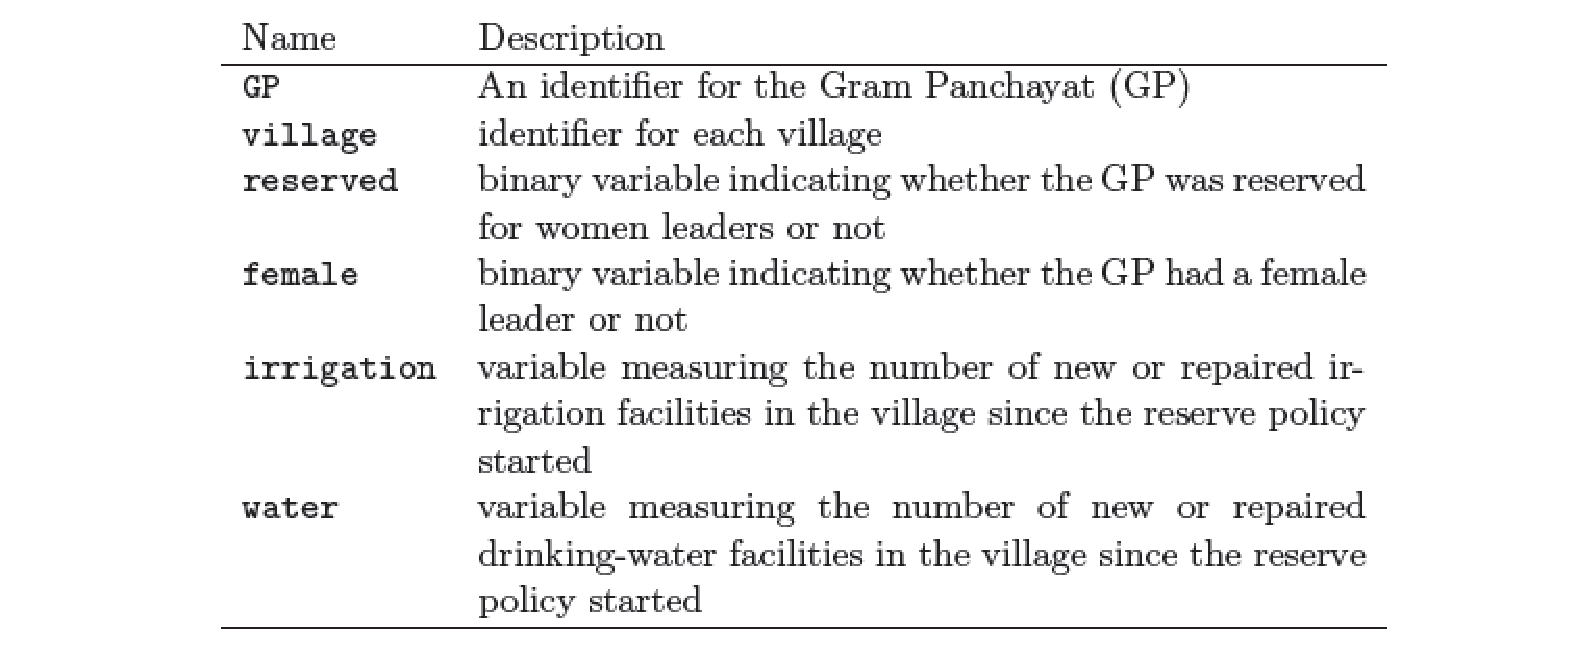
\includegraphics[width=1.1\textwidth]{women_desc.eps}
	\end{figure}		
	
	\newpage
	\begin{enumerate}
		\item [(a)] State a null and alternative (two-tailed) hypothesis. 
		
	\noindent \textbf{Step 1: State Hypotheses}
	\item Null hypothesis: the reservation policy has no correlation with the number of drinking water facilities
    \item Alternative hypothesis: the reservation policy has a correlation with the number of drinking water facilities

		\vspace{1cm}
		\item [(b)] Run a bivariate regression to test this hypothesis in \texttt{R} (include your code!).
	
		\noindent \textbf{Step 2: Run a bivariate regression}
	
		\noindent Use the lm function in R to run the regression, I subset two columns from the \break original data set to input only the two variables that I am investigating the relationship between, reserved and water. With reserved as the explanatory variable and water as the response variable.
		
		\lstinputlisting[language=R, firstline=96, lastline=98]{PS02_answersKC.R}  
		
		\begin{verbatim}
		Call:
		lm(formula = women$water ~ women$reserved)
		
		Coefficients:
		(Intercept)  women$reserved  
		14.738           9.252  
		\end{verbatim}
		
		\newpage
		
		\noindent Summary of the regression output
		
		\lstinputlisting[language=R, firstline=100, lastline=100]{PS02_answersKC.R} 
		
		\begin{verbatim}
Call:
lm(formula = women$water ~ women$reserved)

Residuals:
Min      1Q  Median      3Q     Max 
-23.991 -14.738  -7.865   2.262 316.009 

Coefficients:
               Estimate Std. Error t value Pr(>|t|)    
(Intercept)      14.738      2.286   6.446 4.22e-10 ***
women$reserved    9.252      3.948   2.344   0.0197 *  
---
Signif. codes:  0 ‘***’ 0.001 ‘**’ 0.01 ‘*’ 0.05 ‘.’ 0.1 ‘ ’ 1

Residual standard error: 33.45 on 320 degrees of freedom
Multiple R-squared:  0.01688,	Adjusted R-squared:  0.0138 
F-statistic: 5.493 on 1 and 320 DF,  p-value: 0.0197

		\end{verbatim}
		
		\item [(c)] Interpret the coefficient estimate for reservation policy. 

        \noindent \textbf {Interpret the coefficients}
        
   \begin{itemize}     
        \item A coefficient estimate of 9.252 suggests that for a one unit increase in reservation policy (in this case a one unit increase represents going from no reservation policy to having a reservation policy) there is a 9.252 increase in the number of new or repaired drinking water facilities in the village
        
        \item A p-value of 0.0197 is less than the critical value of 0.05, indicating that we can reject the null hypothesis that there is no relationship between reservation policy and the number of drinking water facilities
        
        \item A y-intercept of 14.738 suggests that we predict 14.738 new or repaired drinking-water facilities when there is no reservation policy in place.
    \end{itemize}
    	
	\end{enumerate}


	
\end{document}
